\chapter{Demonstration} \label{chap:results}
	Thermodynamics plays a central role in driving several physical phenomena and in nuclear it is often used in conjunction with other codes such as phase-field model or fuel performance code. Another very useful application of the thermodynamic equilibrium is to study the behaviour of nuclear fuels and materials under severe accident conditions such as in predicting the impact of oxygen potential on onset temperature of fuel volatilisation. Though the goal of this work was to develop the capability to use thermodynamic equilibrium calculations in modelling nuclear materials, the tool was used to perform several calculations which can demonstrate its capability. It must be emphasised that such calculations are purely intended to demonstrate the capability of the tool developed as part of this research and are not aimed at modelling real-world problems and phenomena. Several such examples are presented in this chapter. The first example demonstrates a simple coupling between {\GEM} and MOOSE phase field module to model leaching of \ce{Ni} by molten \ce{LiF-NiF2} salt. The second example reproduces a couple of phase-diagrams already reported in literature followed by an example of phase evolution of oxide fuel. The last example shows how thermochemical equilibrium calculations may be relevant to source term modelling in MSR. Lastly, a comparison between the calculations from {\GEM} and calculations from the commercial code FactSage are shown as a benchmark.
	
	\section{GEM - Phase Field Coupling}
The objective of {\YJ} development was to allow concurrent coupling of GEM with the phase field module in MOOSE. To achieve this a two step process was adopted. The first step was an offline coupling where {\GEM} calculations are used to pre-tabulate the Gibbs energy and chemical potential data. This data was then used to generate interpolated functions of Gibbs energy and chemical potentials using the \texttt{PiecewiseLinearInterpolationMaterial} object in MOOSE. The interpolated functions were used as material properties in the phase field calculation. In doing so, one must also account for the difference between the Gibbs energies required by the phase field model and those calculated by {\GEM}. The thermodynamic equilibrium calculations compute the Gibbs energy from the MQMQA and are in the following form:
\begin{equation}
	g_\text{GEM} = \sum x_i g_i^\circ + RT\left( \sum x_i \log{x_i} \right) + g^\text{ex},
\end{equation}
where $g^\text{ex}$ is the excess mixing contribution as always. On the other hand, the phase field model requires that the Gibbs energy and chemical potentials also capture the effect of redox reactions and hence the Gibbs energy in phase field module takes the following form:
\begin{equation}
	g_\text{PF} = \sum x_i g_i^\text{ec}  + RT\left( \sum x_i \log{} \right) + g^\text{ex},
\end{equation}
where $g_i^\text{ec}$ denotes the Gibbs energy with the reduction component accounted for. 

For the initial demonstration of the methodology, \ce{LiF-NiF2} salt interacting with $Ni$ metal at \SI{1150}{\kelvin} was selected. The Gibbs energy from the thermodynamic equilibrium code then takes the following form:
\begin{equation*}
	g_\text{GEM} = x_{\ce{NiF2}} g_{\ce{NiF2}}^\circ + x_{\ce{LiF}} g_{\ce{LiF}}^\circ + RT\left( x_{\ce{NiF2}} \log{x_{\ce{NiF2}}} + x_{\ce{LiF}} \log{x_{\ce{LiF}}} \right) + g^\text{ex}.
\end{equation*}
To reduce the number of variables in the phase field model, the reference Gibbs energy of \ce{LiF2} is set to zero. \ce{NiF2} is assumed to be formed from \ce{Ni} metal by reducing   \ce{HF} into \ce{H2} and the Gibbs energy of formation of \ce{NiF2} is then equal to $g_{\ce{NiF2}}^\circ - 2 g_{\ce{HF}}^\circ + g_{\ce{H2}}^\circ + \nu F \Delta E_{\ce{F}}$. This gives the following Gibbs energy expression for the phase field model
\begin{equation*}
	g_\text{PF} = x_{\ce{NiF2}} \left( g_{\ce{NiF2}}^\circ - 2 g_{\ce{HF}}^\circ + g_{\ce{H2}}^\circ + \upsilon F \Delta E_{\ce{F}} \right) + RT\left( x_{\ce{NiF2}} \log{x_{\ce{NiF2}}} + x_{\ce{LiF}} \log{x_{\ce{LiF}}} \right) + g^\text{ex},
\end{equation*}
where $\upsilon$ represents the valency (2 for \ce{Ni^{2+}}), $F$ is Faraday's constant and $\Delta E_{\ce{F}}$ denotes the fluoride potential of the salt. The fluoride potential is calibrated based on the experimental data and represents how oxidising the environment is (higher $\Delta E_{\ce{F}}$ is less oxidising). To use {\GEM} calculations in the phase field model, the Gibbs energy can then be reconciled as follows:
\begin{equation*}
	g_\text{PF} = g_\text{GEM} - x_{\ce{NiF2}} \left( 2 g_{\ce{HF}}^\circ - g_{\ce{H2}}^\circ - g_{\ce{LiF}}^\circ - \nu F \Delta E_{\ce{F}} \right).
\end{equation*}

A phase field simulation was performed at the University of Florida\footnote{The phase field calculations were performed by Chaitanya Bhave, University of Florida.} to demonstrate the potential of coupling the Gibbs energy minimiser with the phase field model. The reference phase field model used the Nernst equation for the Gibbs energy equation which does not capture the excess mixing contribution. As shown in figure~\ref{fig:pfgibbs}, the use of GEM allowed capturing the excess mixing effects which were not captured previously. While the difference for the binary system considered was relatively small, the excess mixing contributions for larger systems such as ones with impurities can be significant and being able to capture the additional contributions can significantly improve the fidelity of phase field models.
    \begin{figure}[h!]
        \centering
        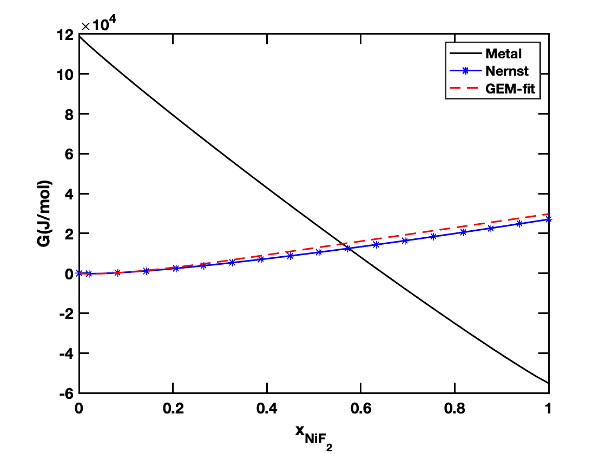
\includegraphics[width=0.75\textwidth]{figures/chapter-7/gibbs.png}
        \caption{Comparison of Gibbs energy predicted by the Gibbs energy minimiser vs. the dilute Nernst energy model used previously.}
        \label{fig:pfgibbs}
    \end{figure}

\ce{Ni} leaching with molten \ce{LiF-NiF2} was simulated under two conditions - $\Delta E_{\ce{F}} = 2.871$ \si{\volt} which represents oxidising conditions and $\Delta E_{\ce{F}} = 3.0$ \si{\volt} which represents reducing conditions. The mole fraction of \ce{Ni} in the molten salt phase was fixed as $x_{\ce{Ni}} = 0.001$. The results of \ce{Ni} leaching have been shown in figures~\ref{fig:pfres2} and \ref{fig:pfres3}. Under oxidising conditions \ce{Ni} metal gets leached into the molten salt and the interface moves to the left as shown in figure~\ref{fig:pfres2} while the opposite happens under reducing conditions as shown in  figure~\ref{fig:pfres3}. 
\begin{figure}[!ht]
    \subfloat[Start of simulation\label{fig:EF2_i}]{%
      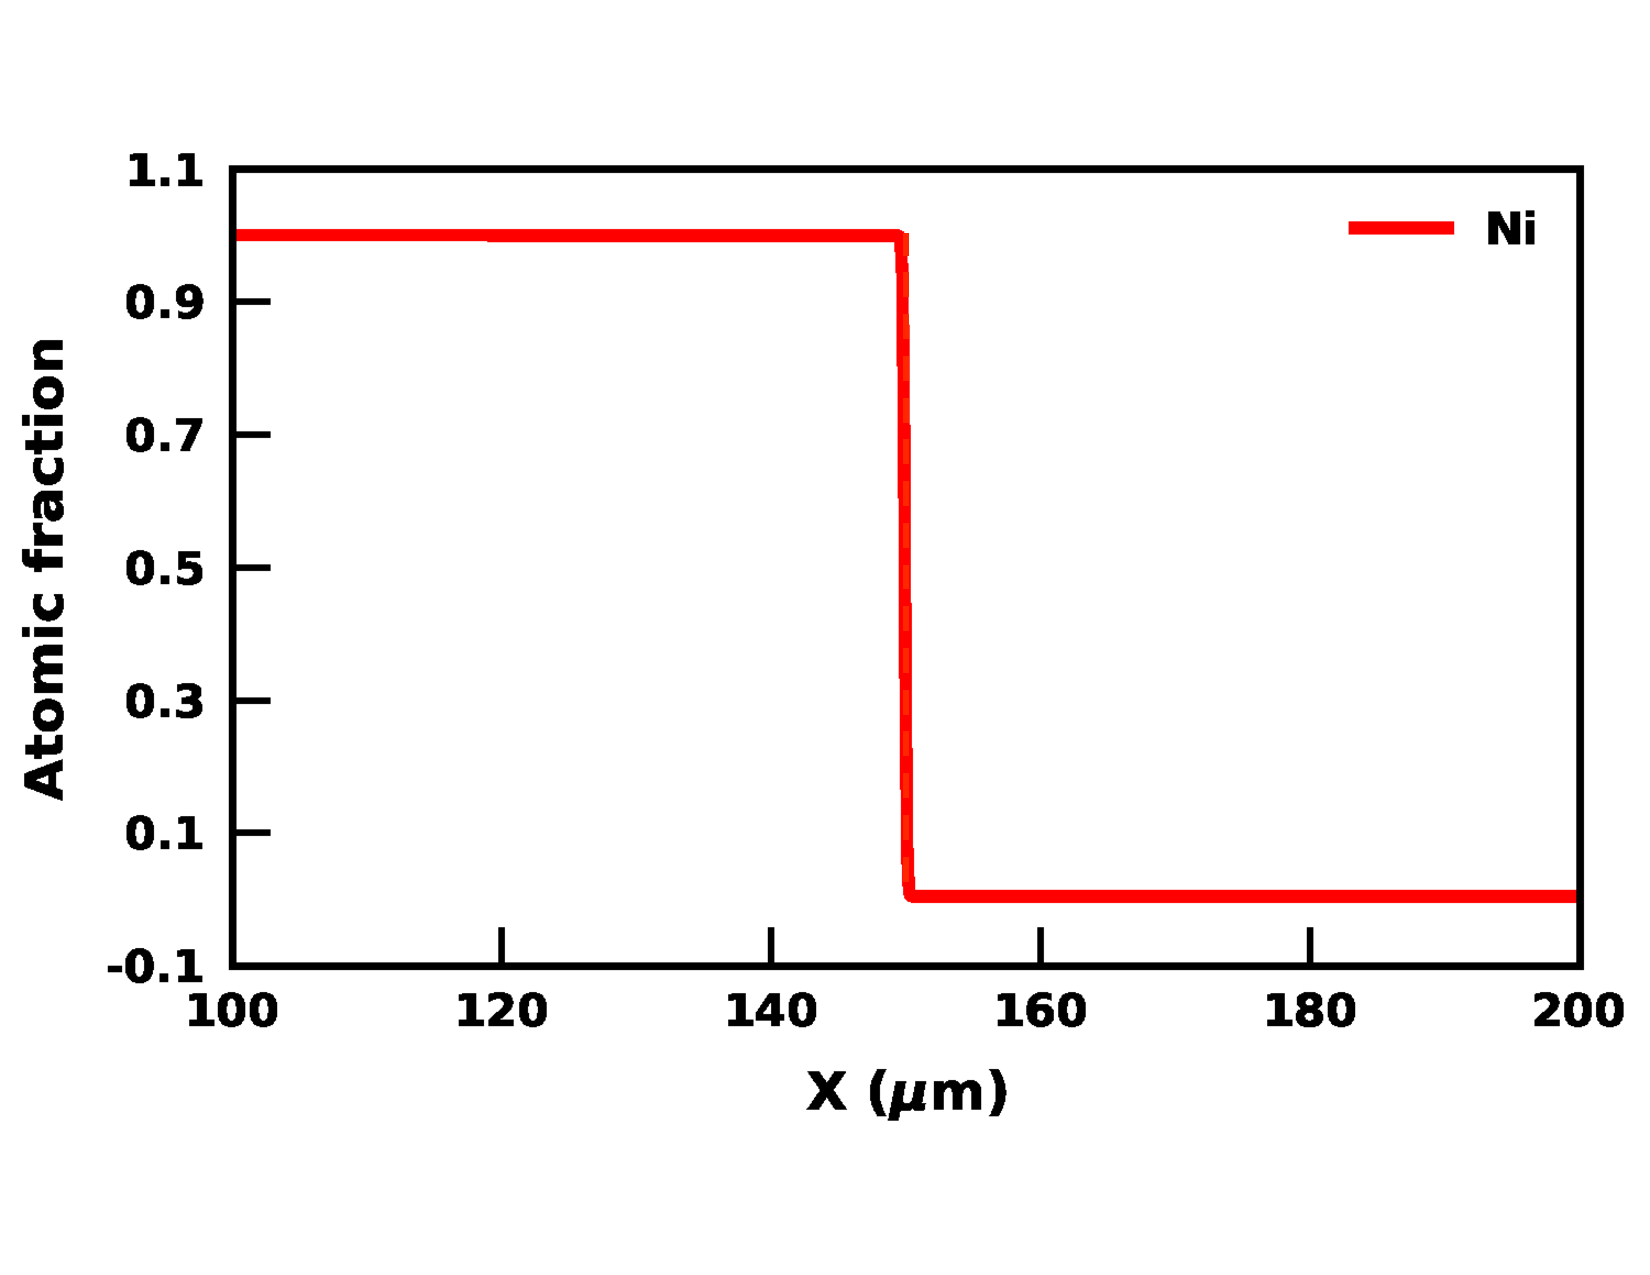
\includegraphics[width=0.475\textwidth]{figures/chapter-7/EF_2.871_i.pdf}
    }
    \hfill
    \subfloat[End of simulation\label{fig:EF2_e}]{%
      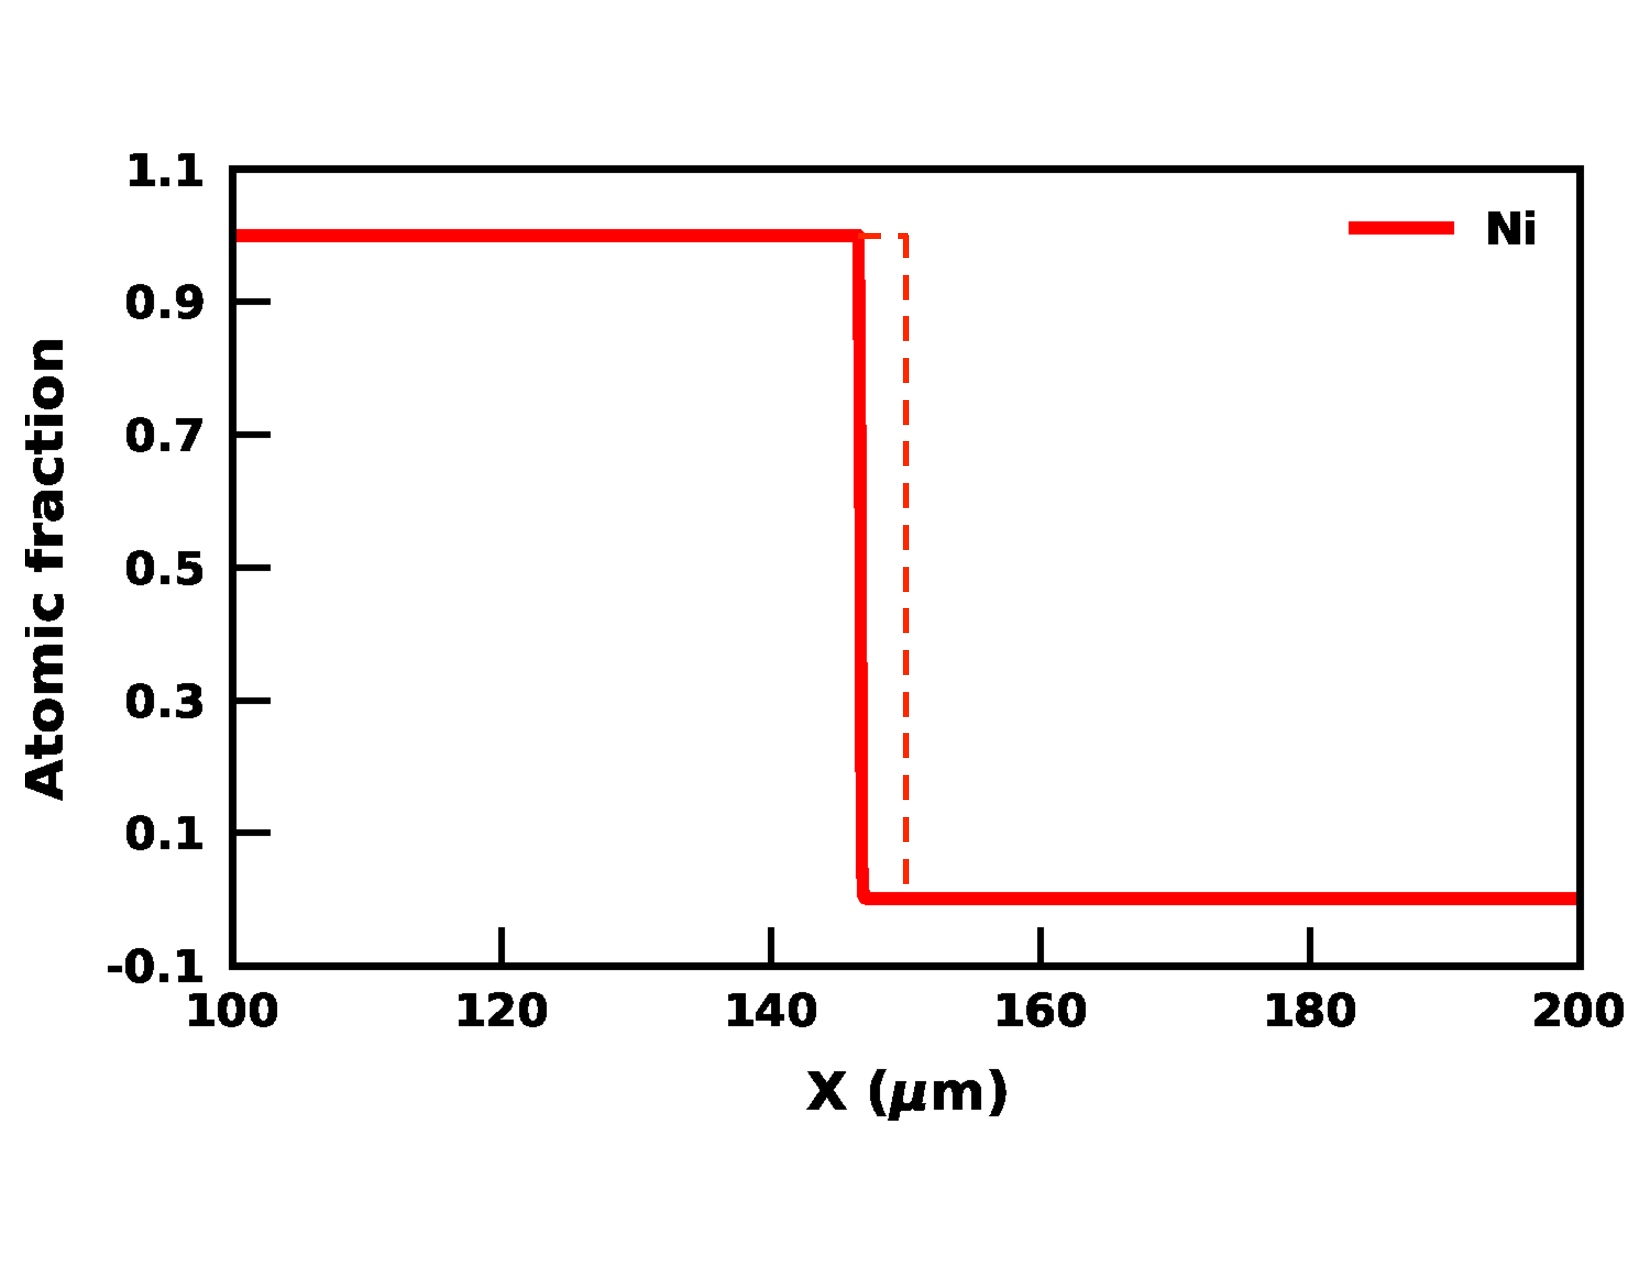
\includegraphics[width=0.475\textwidth]{figures/chapter-7/EF_2.871_e.pdf}
    }
    \caption[Simulation of \ce{Ni} corrosion by \ce{LiF-NiF2} salt under oxidising condition $\left(\Delta E_{\ce{F}} = 2.871\right)$.]{Simulation of \ce{Ni} corrosion by \ce{LiF-NiF2} salt under oxidising condition $\left(\Delta E_{\ce{F}} = 2.871\right)$. Initially, the domain contained \ce{Ni} in the left half of the domain and molten salt in the right half as in subfigure (a). At the end of the simulation shown in subfigure (b), the oxidation of \ce{Ni} metal leads to the leaching of \ce{Ni} into the molten salt as exhibited by the interface shifting to the left (the dashed line denotes the initial position of interface).}
    \label{fig:pfres2}
\end{figure}

\begin{figure}[!ht]
    \subfloat[Start of simulation\label{fig:EF3_i}]{%
      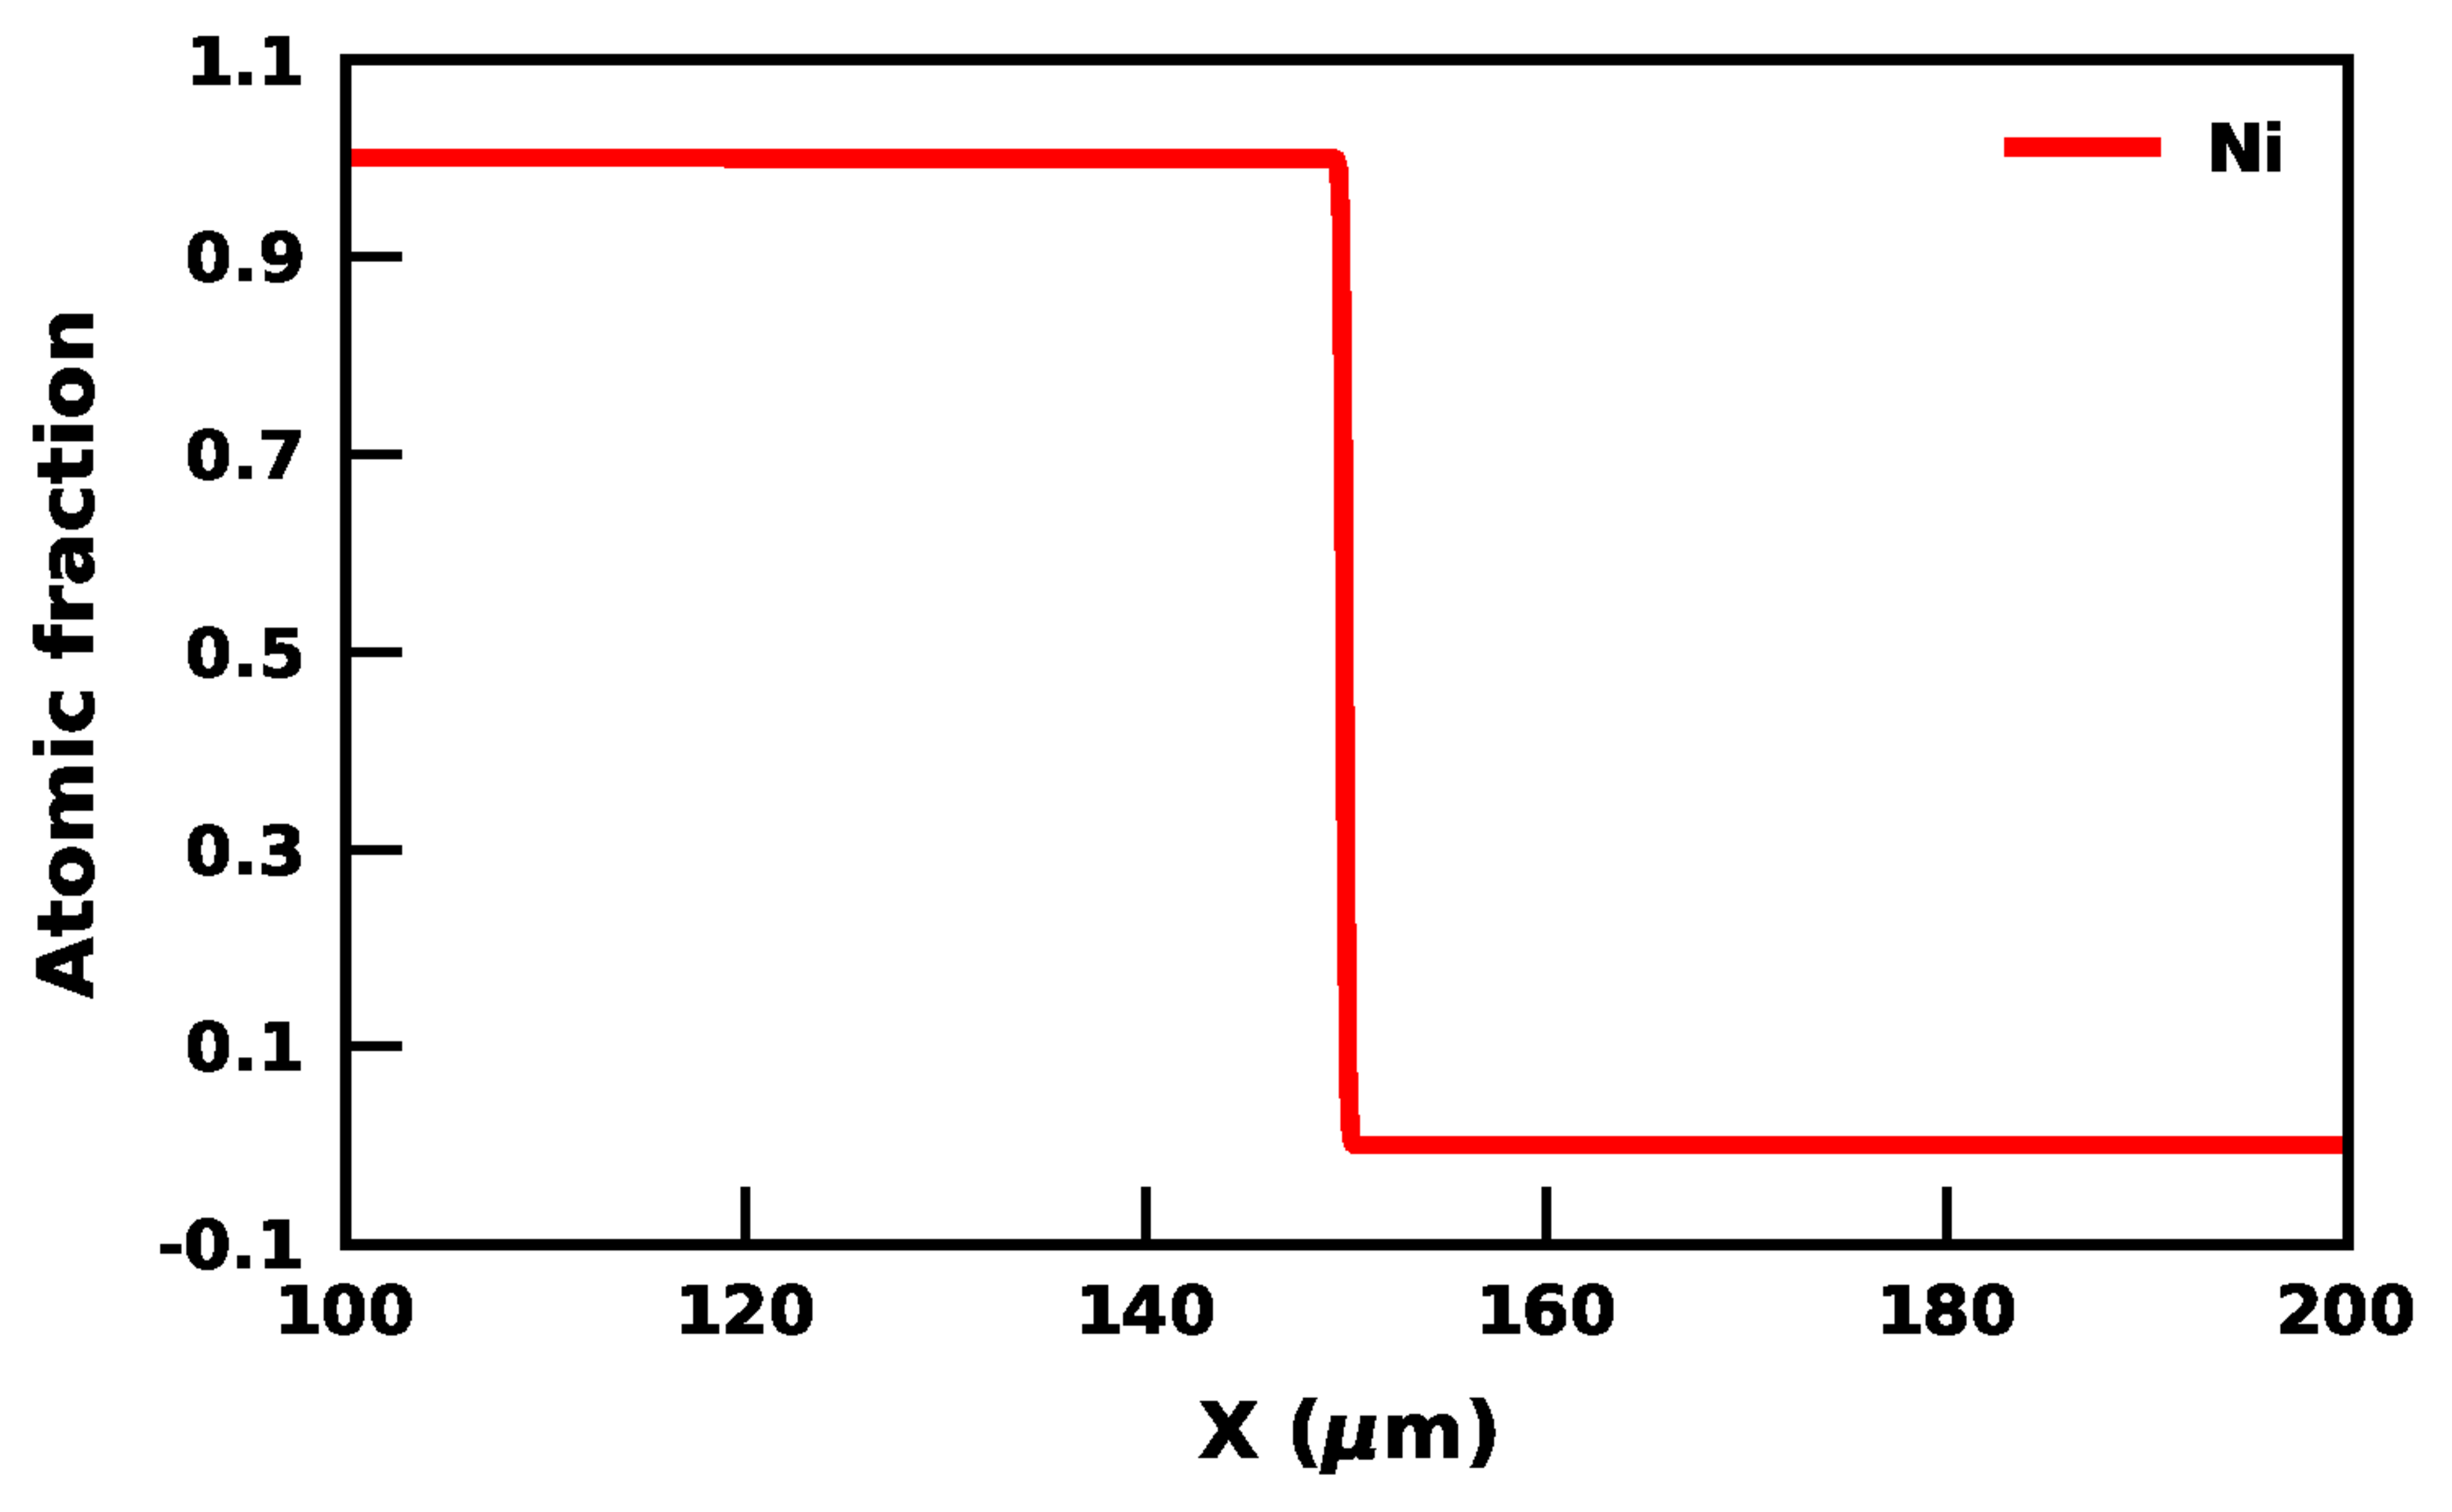
\includegraphics[width=0.475\textwidth]{figures/chapter-7/EF_3.0_i.pdf}
    }
    \hfill
    \subfloat[End of simulation\label{fig:EF3_e}]{%
      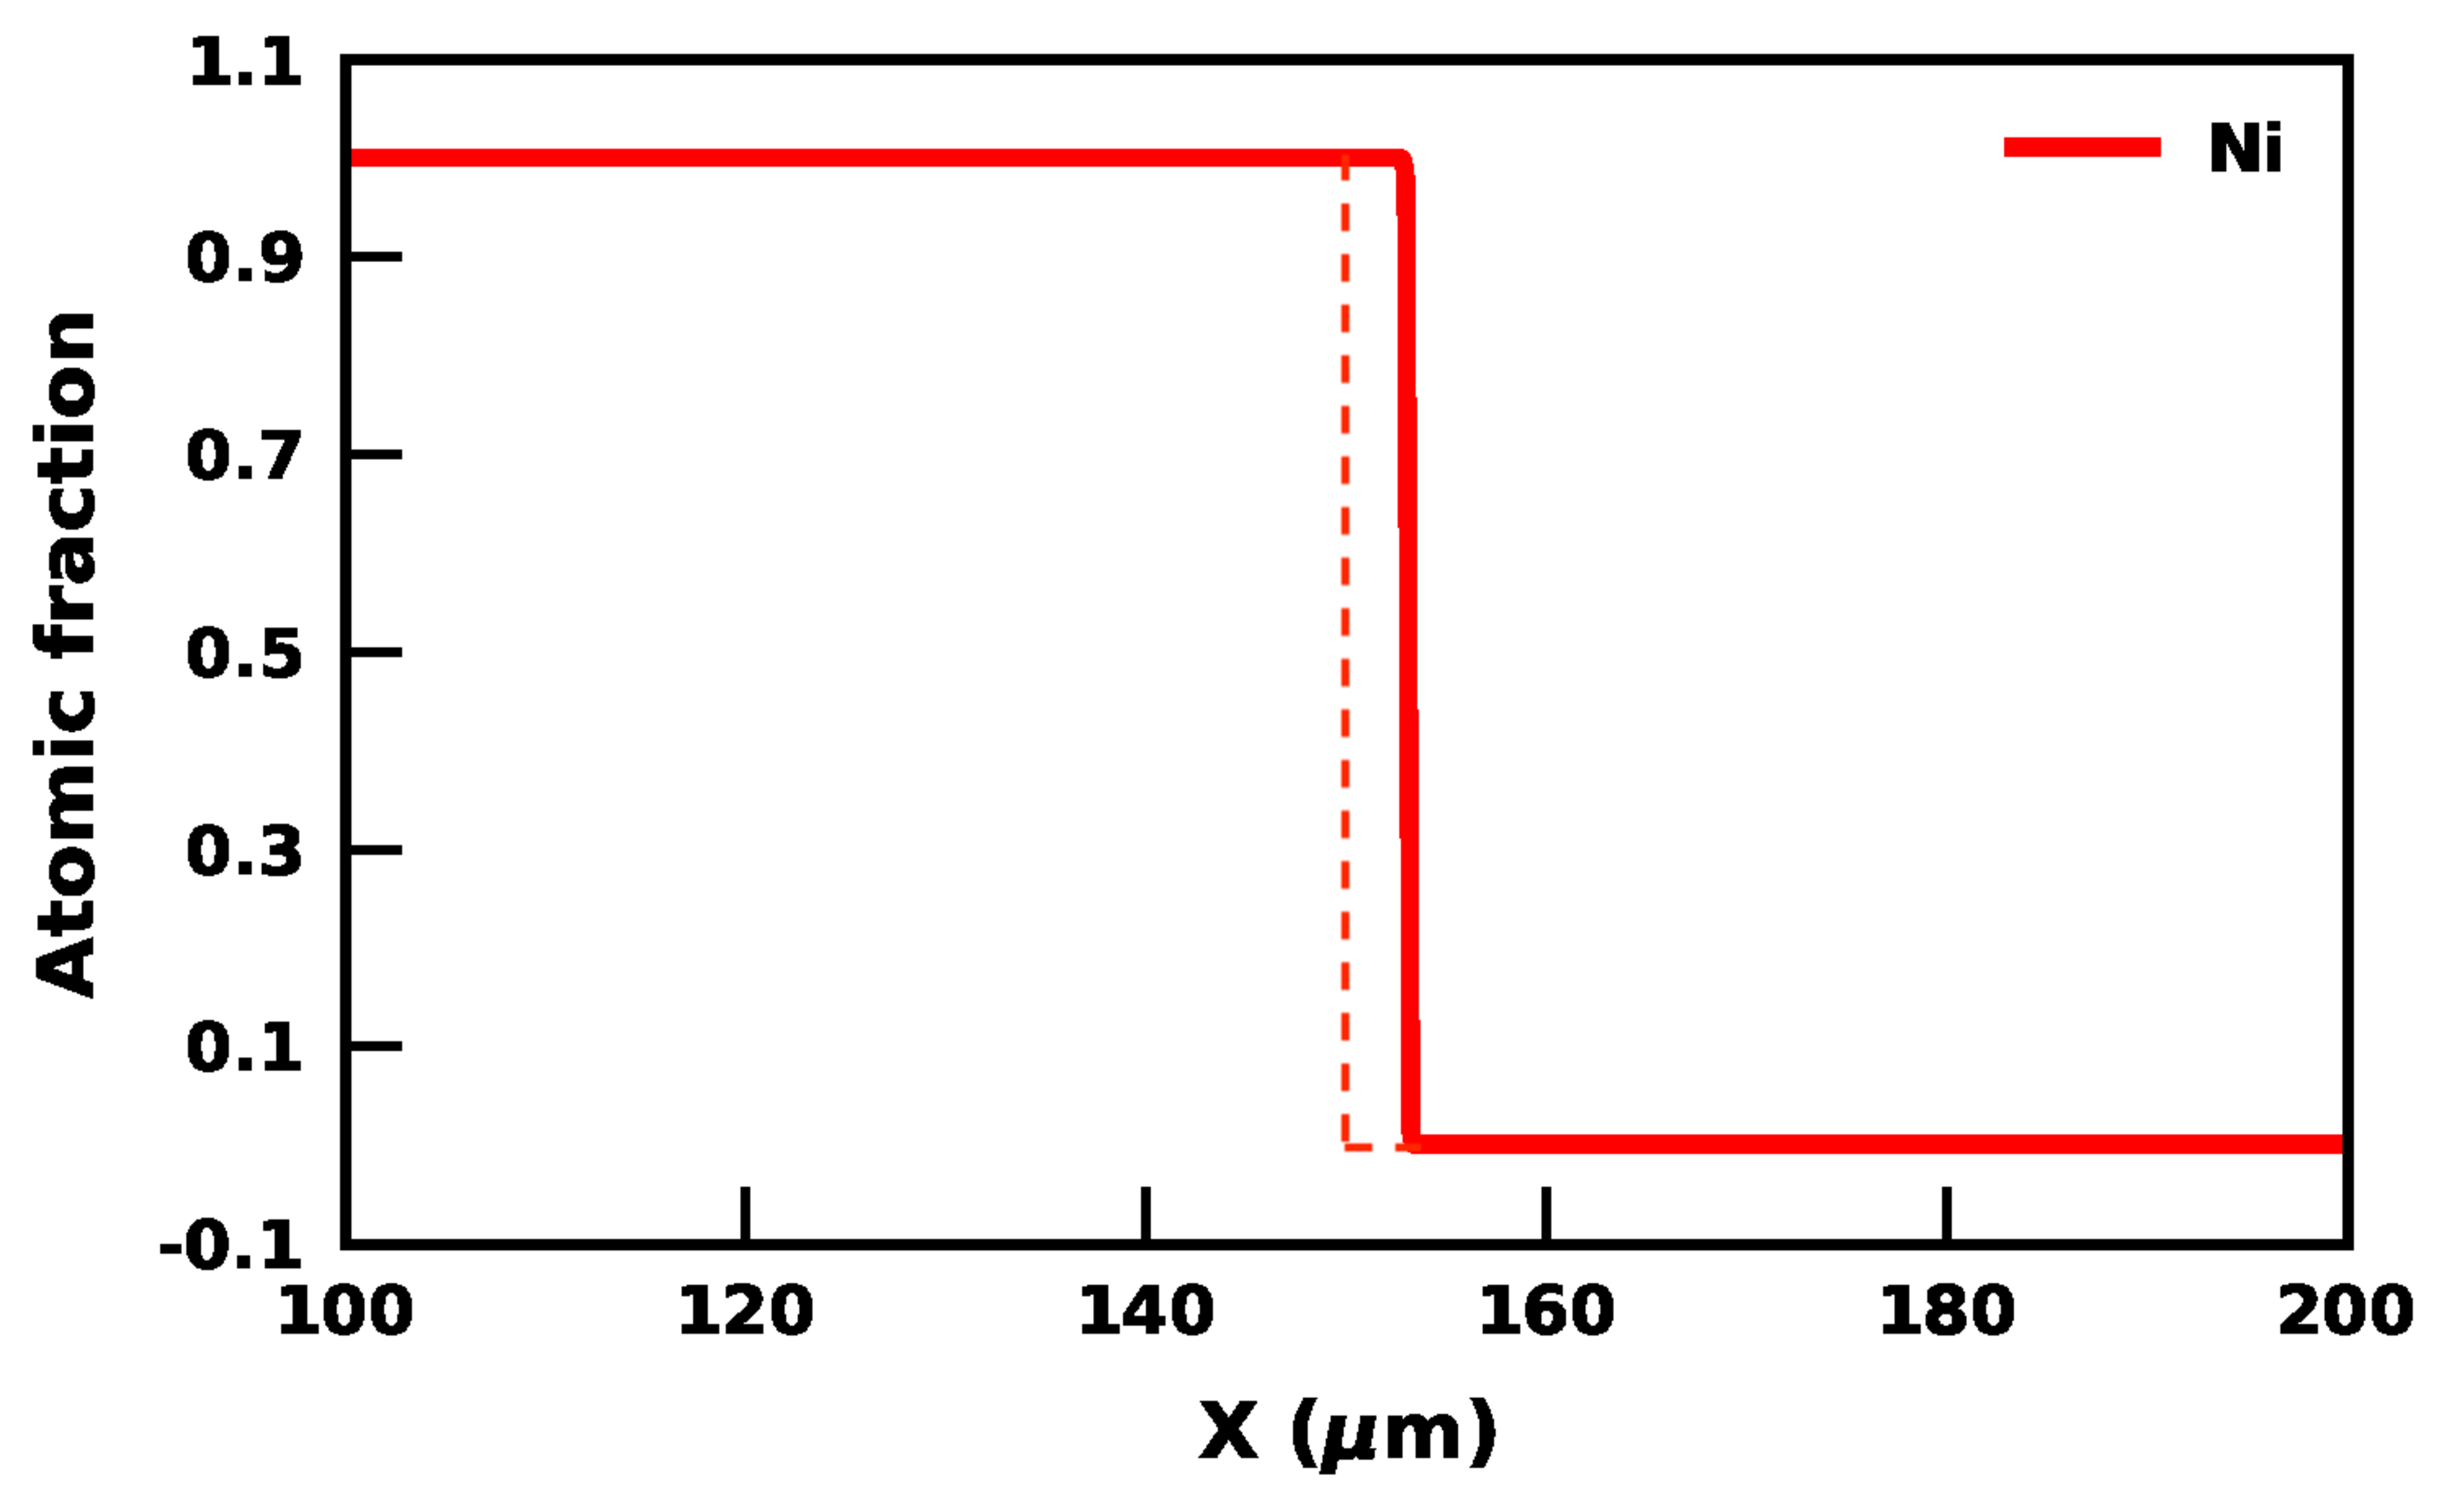
\includegraphics[width=0.475\textwidth]{figures/chapter-7/EF_3.0_e.pdf}
    }
    \caption[Simulation of \ce{Ni} corrosion by \ce{LiF-NiF2} salt under reducing condition $\left(\Delta E_{\ce{F}} = 3.0\right)$.]{Simulation of \ce{Ni} corrosion by \ce{LiF-NiF2} salt under reducing condition $\left(\Delta E_{\ce{F}} = 3.0\right)$. The initial interface is shown in subfigure (a) while at the end of the simulation shown in subfigure (b), the reduction of \ce{Ni} metal leads to gain of \ce{Ni} metal from the molten salt as exhibited by the interface shifting to the right (the dashed line denotes the initial position of interface).}
    \label{fig:pfres3}
\end{figure}
       
\section{Phase Diagram Construction}
	Thermodynamic equilibrium calculations form the basis of phase diagram calculation. To demonstrate such applications, the \ce{NaF-CsF} binary system was phase diagram was calculated using {\GEM}. This binary system has been recently re-evaluated experimentally by Lipkina et al. \cite{Lipkina:2022aa} and the phase diagram generated here was compared to the experimental results. The calculations from {\GEM} are shown in figure~\ref{fig:res_phased} and show excellent agreement with the experimental data for the eutectic points. There is, however, a departure between the liquidus points calculated by Lipkina et al. and the ones predicted by {\YJ}. This is a direct consequence of the database used in the calculations (MSTDB-TC) as it has not been updated to reflect the recent experimental results. In fact, as shown by the solid black line, the calculations match the results of the previously available experimental data. The example not only highlights the capability of {\GEM} but also shows a need for the re-evaluation of the \ce{NaF-CsF} thermodynamic model currently used in the databases.
\begin{figure}
         \centering
         \includegraphics[width=0.95\textwidth]{figures/chapter-7/phasedia.png}
 	 \caption{Yellowjacket prediction of \ce{NaF-CsF} phase diagram with the phase diagram from Lipkina et al. \cite{Lipkina:2022aa} overlayed on top.}
	 \label{fig:res_phased}
\end{figure}
\begin{figure}
         \centering
         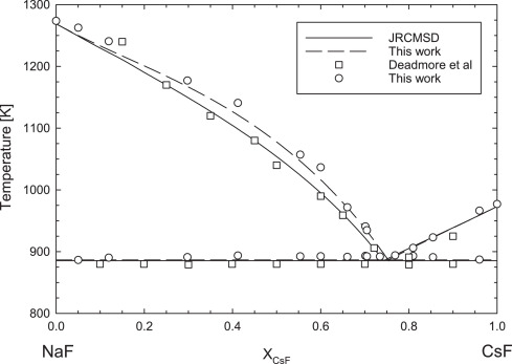
\includegraphics[width=0.7\textwidth]{figures/chapter-7/pdo.png}
         \caption[Reference \ce{NaF-CsF} phase  diagram from Lipkina et al.]{Reference \ce{NaF-CsF} phase  diagram from Lipkina et al. \cite{Lipkina:2022aa}.}
     \label{fig:res_refdia}
\end{figure}

\section{CANDU Fuel Phase Evolution}
Severe accident scenarios are amongst the phenomena which benefit most from the use of thermodynamic equilibrium calculations. Piro performed thermodynamic investigations on irradiated uranium dioxide CANDU fuel under conditions representative of severe accident scenarios \cite{Piro:2022aa}. Piro considered two cases of irradiated fuel interacting with the atmosphere. In the first case, the fuel was in contact with hydrogen gas while in the second case the irradiated fuel was in contact with air and steam.  Piro used TAF-ID \cite{Gueneau15,Gueneau:2021aa} and varied the ratio of fuel to total atmospheric gas as well as the temperature and hydrostatic pressure. Here, a couple of similar simulations are performed albeit for the first case with a single fuel to atmosphere ratio and the database used is a modified version of TAF-ID obtained by translating the TAF-ID tdb file into ChemSage format. For the simulation, the same composition as that used by Piro was selected and the values are reported in table~\ref{tab:composition_candu}. In the table, $b_{\ce{O}}$, $b_{\ce{H}}$ and $b_{\ce{N}}$ are variables which depend on the hydrogen to steam molar ratio $H = n_{\ce{H2}} / n_{\ce{H2O}}$, air to steam molar ratio $A = n_{\text{air}} / n_{\ce{H2O}}$, and fission product to atmosphere molar ratio $R = b_{\ce{Cs}} / n_{\text{gas}}$. The calculations show that under the given conditions, the main phase is O2ZRU\_C with other phases evolving as the system temperature changes. It must again be emphasised that the simulation is only representative of the capabilities developed as part of {\GEM} and must be considered as a safety case simulation. 
\begin{table}[htb]
		\centering
	   	\caption[Input mass parameters for CANDU fuel under severe accident condition.]{Input mass parameters for CANDU fuel under severe accident condition. Adopted from Piro \cite{Piro:2022aa}.}
	   	\begin{tabular}{@{} lcr @{}} % Column formatting, @{} suppresses leading/trailing space
	      		\toprule
	      		\textbf{Element} & \phantom{abc}& \textbf{Moles [\si{\mole}]} \\
	      		\midrule
	      		\ce{O}	& & $b_{\ce{O}}$\\
			\ce{U}	& & \num{1014.5}\\
			\ce{Np}	& & \num{0.096}\\
			\ce{Pu}	& & \num{2.754}\\
			\ce{Ce}	& & \num{0.824}\\
			\ce{Y}	& & \num{0.215}\\
			\ce{Te}	& & \num{0.138}\\
			\ce{La}	& & \num{0.332}\\
			\ce{Zr}	& & \num{1.442}\\
			\ce{Ba}	& & \num{0.389}\\
			\ce{Ru}	& & \num{0.899}\\
			\ce{Mo}	& & \num{1.15}\\
			\ce{Sr}	& & \num{0.421}\\
			\ce{I}		& & \num{0.077}\\
			\ce{Nd}	& & \num{0.859}\\
			\ce{Nb}	& & \num{0.043}\\
			\ce{Am}	& & \num{0.0064}\\
			\ce{Cs}	& & \num{0.745}\\
			\ce{Rh}	& & \num{0.166}\\
			\ce{H}	& & $b_{\ce{H}}$\\
			\ce{N} 	& & $b_{\ce{N}}$\\
	      		\bottomrule
	   \end{tabular}
	   \label{tab:composition_candu}
	\end{table}

Using $H = 10^5$ and $R = 10^{-4}$ for the case of fuel in contact with hydrogen, $b_{\ce{O}} = 2029.07449$ and $b_{\ce{H}} = 14900.00$. With the hydrostatic pressure $P = 1$ \si{\atmosphere}, the temperature of the system was varied from \SI{1000}{\kelvin} to \SI{3000}{\kelvin} in steps of \SI{50}{\kelvin}. The phase evolution predicted by {\GEM} is shown in figure~\ref{fig:candu_phase}. 
\begin{figure}[ht]
         \centering
         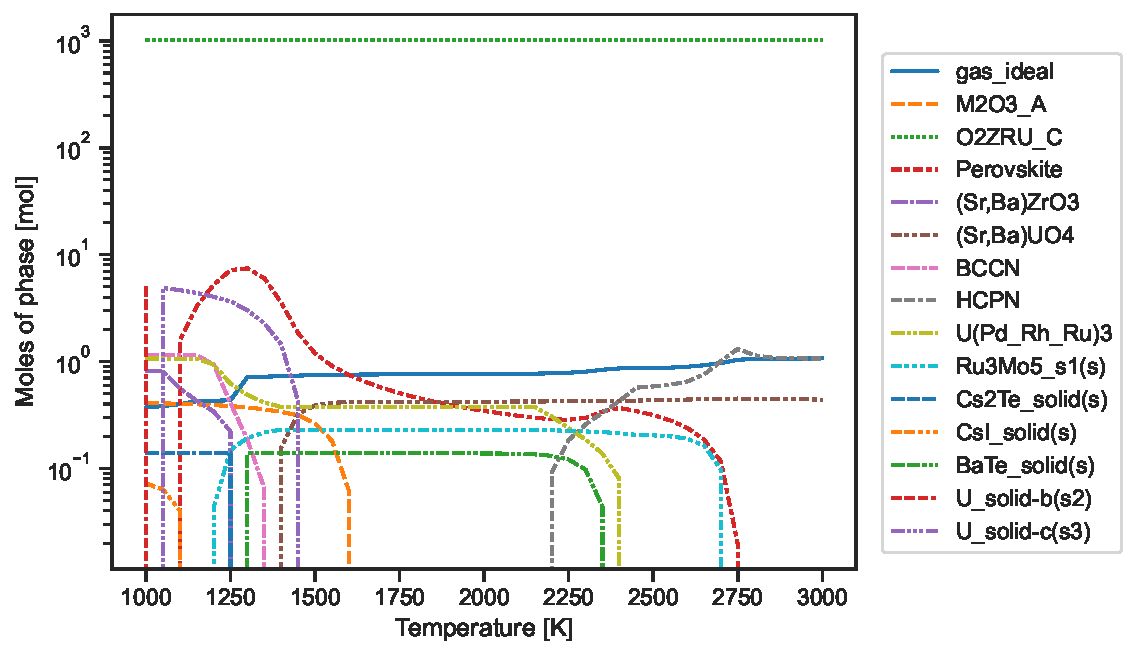
\includegraphics[width=0.95\textwidth]{figures/chapter-7/Candu_moles.pdf}
         \caption{Predicted phase distribution with respect to temperature $H = 10^5$, $R = 10^{−4}$, and $P = 1$ \si{\atmosphere}.}
     \label{fig:candu_phase}
\end{figure}

In addition to comparing phase distributions under the varying system parameters, one is often interested in the oxidation states of different phases as they affect the material properties. Thermodynamic equilibrium calculations can be used to compute the oxygen-to-metal ratio $\left(O/M\right)$ of the phases. The same calculations as those used for the phase evolution were used to calculate the $\left(O/M\right)$ ratio and its evolution for O2ZRU\_C phase is shown in figure~\ref{fig:candu_om}.
\begin{figure}[htb]
         \centering
         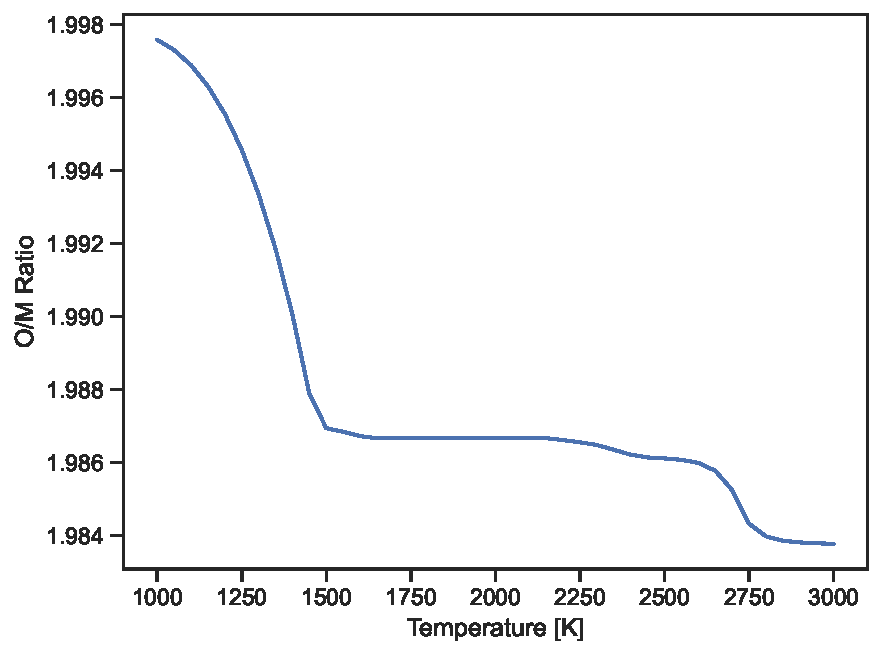
\includegraphics[width=0.9\textwidth]{figures/chapter-7/Candu_OM.pdf}
         \caption{Predicted oxygen-to-metal ratio $\left(O/M\right)$ for O2ZRU\_C phase with respect to temperature $H = 10^5$, $R = 10^{−4}$, and $P = 1$ \si{\atmosphere}.}
     \label{fig:candu_om}
\end{figure}

 
\section{Vapour Pressure Evolution in MSR}
	Safety case demonstrations for MSRs are significantly different from the LWRs. Since the fuel is already molten, there are no thresholds for a major release of radioactive material with severe core damage in MSR accidents. The consequences of a primary system breach depend on the size and breach location and how much of the fuel salt or fission gases are leaked into a confined space.  A small breach can result in significant fuel salt release and the high salt temperature can lead to a high pressure in the confined space  \cite{Holcomb:2021aa}. Predicting vapour pressures is important for such safety demonstrations, but also for design and development of off-gas treatment system. {\GEM} can predict the change of vapour pressure of elements in gas phase which can be used in source-term analyses and other simulations.  The role of thermodynamic equilibrium solver in such cases can be demonstrated by the evolution of a fictive system representative of a molten salt system (\ce{FLiBe}) with some dissolved fissile material (\ce{U}) and some fission products (\ce{Nd, Ce, La, Cs, Rb}).  The system composition was adopted from Poschmann et al. \cite{Poschmann:2021ab} and is reported in table~\ref{tab:composition_msr}.
	\begin{table}[htb]
		\centering
	   	\caption[Input mass parameters for CANDU fuel under severe accident condition.]{Input mass parameters for CANDU fuel under severe accident condition. Adopted from Poschmann et al. \cite{Poschmann:2021ab}.}
	   	\begin{tabular}{@{} lcr @{}} % Column formatting, @{} suppresses leading/trailing space
	      		\toprule
	      		\textbf{Element} & \phantom{abc}& \textbf{Moles [\si{\mole}]} \\
	      		\midrule
	      		\ce{Pu}	& & \num{1.9780d-1}\\
			\ce{U}	& & \num{9.9695d3}\\
			\ce{Nd}	& & \num{3.3553d-1}\\
			\ce{Ce}	& & \num{4.2081d-1}\\
			\ce{La}	& & \num{1.4912d-1}\\
			\ce{Cs}	& & \num{4.2326d-1}\\
			\ce{Rb}	& & \num{8.1960d-2}\\
			\ce{F}	& & \num{4.4d5}\\
			\ce{Be}	& & \num{1.0d5}\\
			\ce{Li} 	& & \num{2.0216d5}\\
	      		\bottomrule
	   \end{tabular}
	   \label{tab:composition_msr}
	\end{table}

The system was assumed to undergo an unmitigated increase in temperature. The phase evolution, vapour pressure of species in gas phase and element potential change as a function of temperature are shown in figures~\ref{fig:res_molemsr}, \ref{fig:res_vpmsr} and \ref{fig:res_epmsr}.
\begin{figure}[ht]
     \centering
     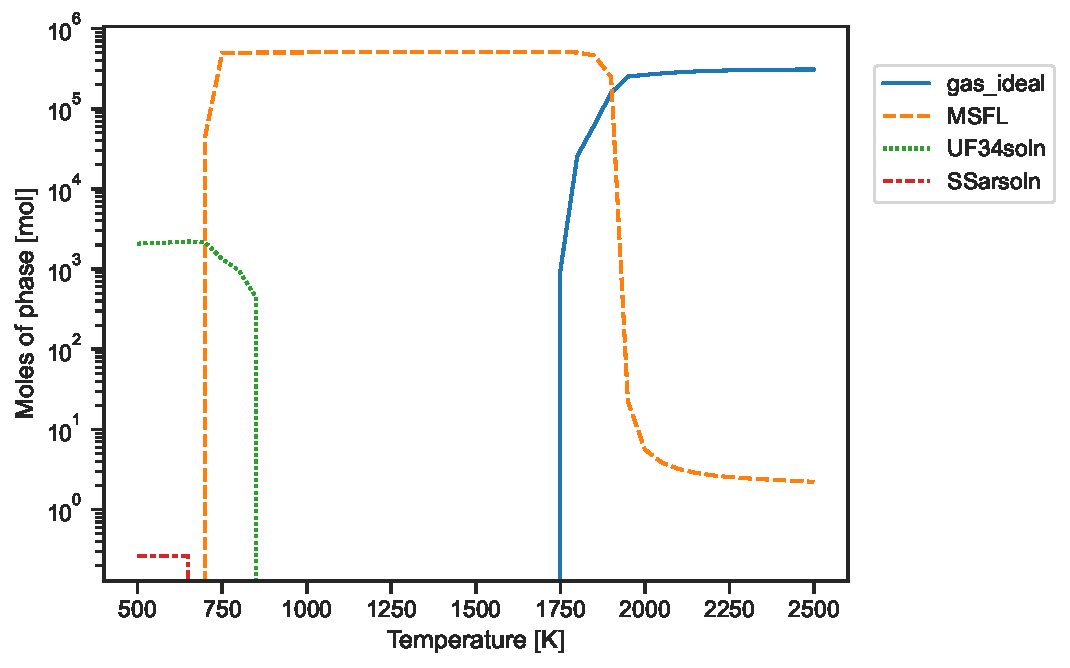
\includegraphics[width=0.9\textwidth]{figures/chapter-7/msr_moles.pdf}
     \caption{Phase evolution in molten salt system.}
     \label{fig:res_molemsr}
\end{figure}
\begin{figure}[ht]
     \centering
     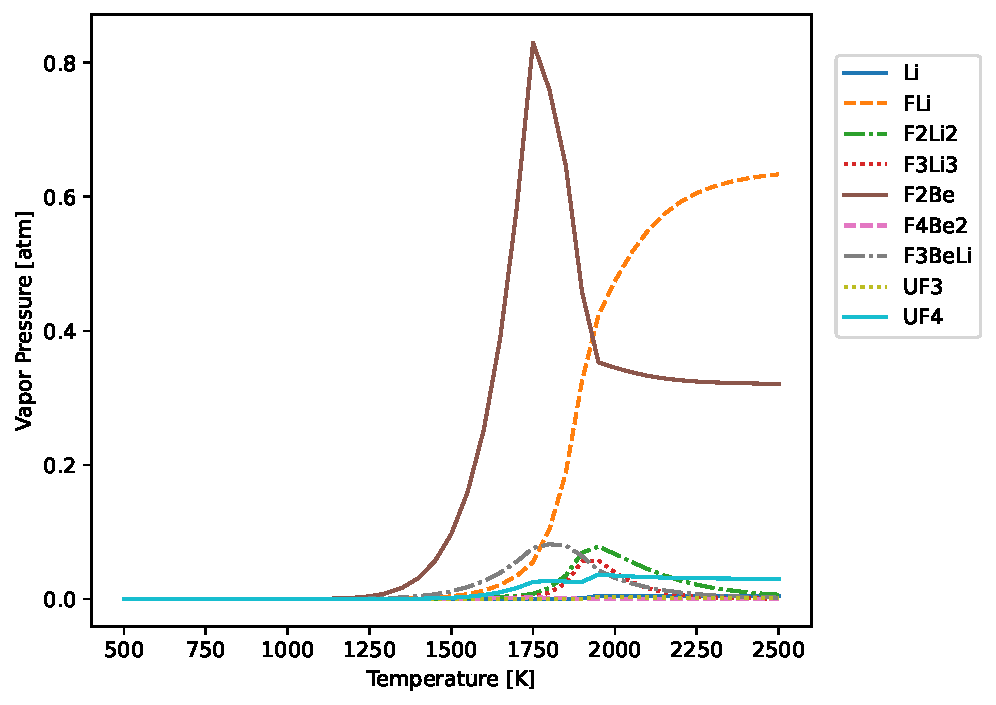
\includegraphics[width=0.9\textwidth]{figures/chapter-7/msr_vp.pdf}
     \caption{Vapour pressure prediction in molten salt system.}
     \label{fig:res_vpmsr}
\end{figure}
\begin{figure}[ht]
         \centering
         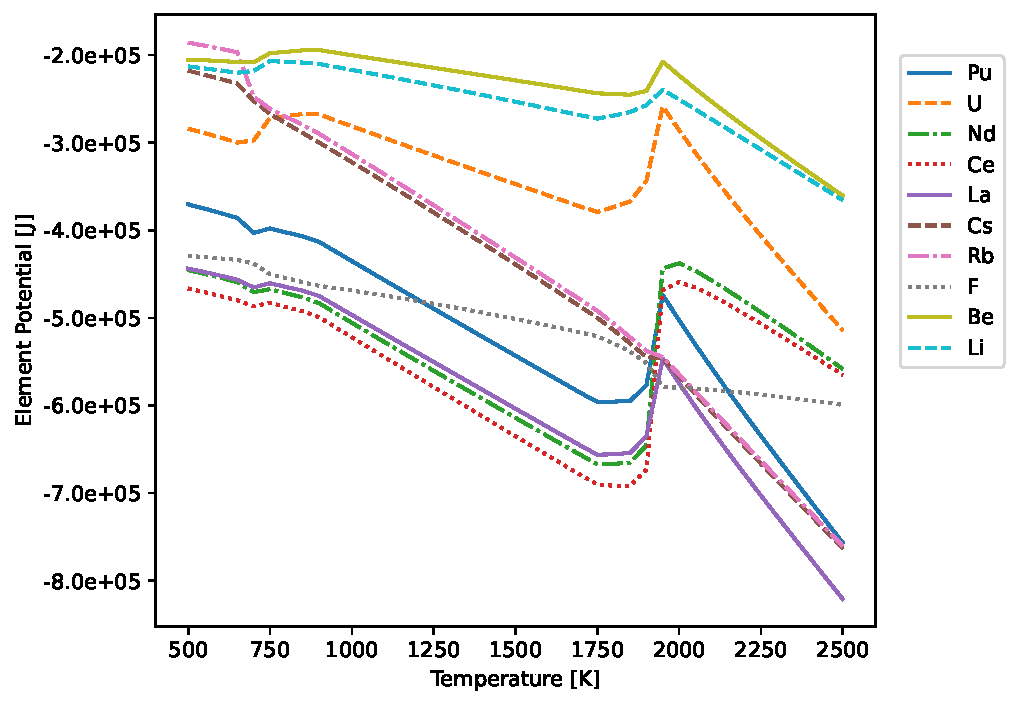
\includegraphics[width=0.9\textwidth]{figures/chapter-7/msr_ep.pdf}
         \caption{Element potential evolution in MSR.}
         \label{fig:res_epmsr}
 \end{figure}
To reiterate, one must note that the results are purely for capability demonstration and must not be treated as physically relevant. However, they do exhibit cases where one might find the use of {\GEM} relevant.
 
\section{Verification}
To ensure the accuracy of results, a significant effort was put into verification of {\GEM} results by comparison with commercial code FactSage. For this, a representative system was selected (the system composition is the same as that used by Poschmann et al. \cite{Poschmann:2021ab}) and the relative difference of the mole fractions of each quadruplet was compared between {\GEM} and FactSage. As shown in figure~\ref{fig:verif}, the results are in excellent agreement with FactSage and the maximum relative difference is of the order of \num{1d-5}. The Gibbs energy predicted by both {\GEM} and FactSage are both \SI{-2.9787d11}{\joule}. 
\begin{figure}[!ht]
    \subfloat[Start of simulation\label{fig:verif_sp}]{%
      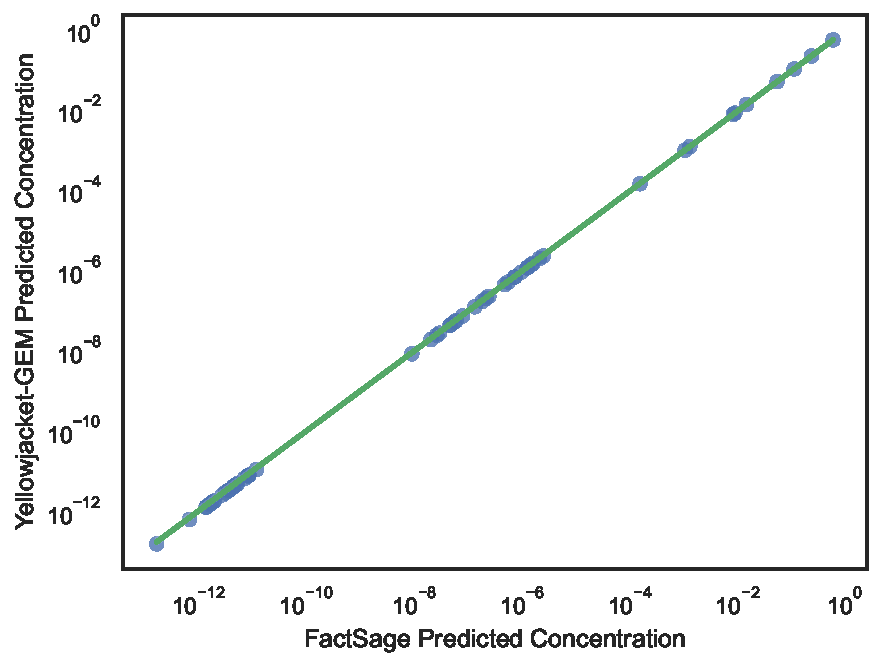
\includegraphics[width=0.5\textwidth]{figures/chapter-7/MQM_Vsp.pdf}
    }
    \hfill
    \subfloat[Quadruplet errors\label{fig:verif_hm}]{%
      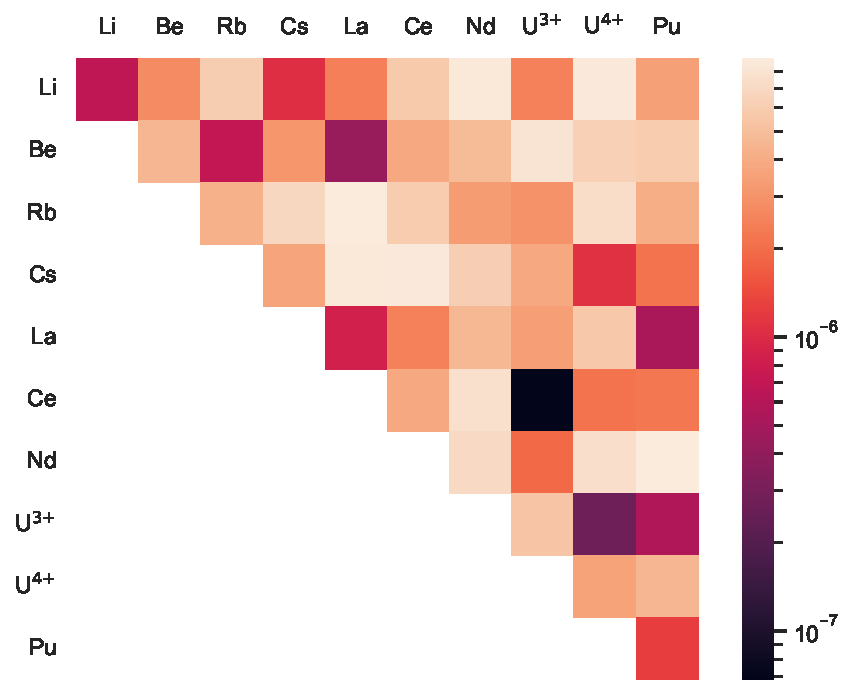
\includegraphics[width=0.46\textwidth]{figures/chapter-7/MQM_Vhm.pdf}
    }
    \caption[Comparison of output species concentrations predictions from {\GEM} and FactSage for the MSR system.]{Comparison of output species concentrations predictions from {\GEM} and FactSage for the MSR system. The figure on the left shows the comparison of the values from the two plots with the green line indicating same values. A more detailed error heatmap is shown on the right with each block denoting the relative error of a quadruplet.}
    \label{fig:verif}
\end{figure}

